\section{Simulation Analysis}
\label{sec:simulation}

For the simulation, NGSpice was used.

An ideal transformer model was used, by implementing a dependent current source and a dependent voltage source. 

The values of n (dependent sources dependency parameter), the resistance and the capacitance were adjusted throughout the preparation of the assignment in order to achieve the maximum accuracy of the desired output voltage of 12V.

The input voltage of the dependent voltage source, vr, the output voltage of the envelope detector, v(4), and the output voltage of the voltage regulator, v(5), were all computed and are presented in Figure~\ref{fig:sim3a}.


\begin{figure}[h] \centering
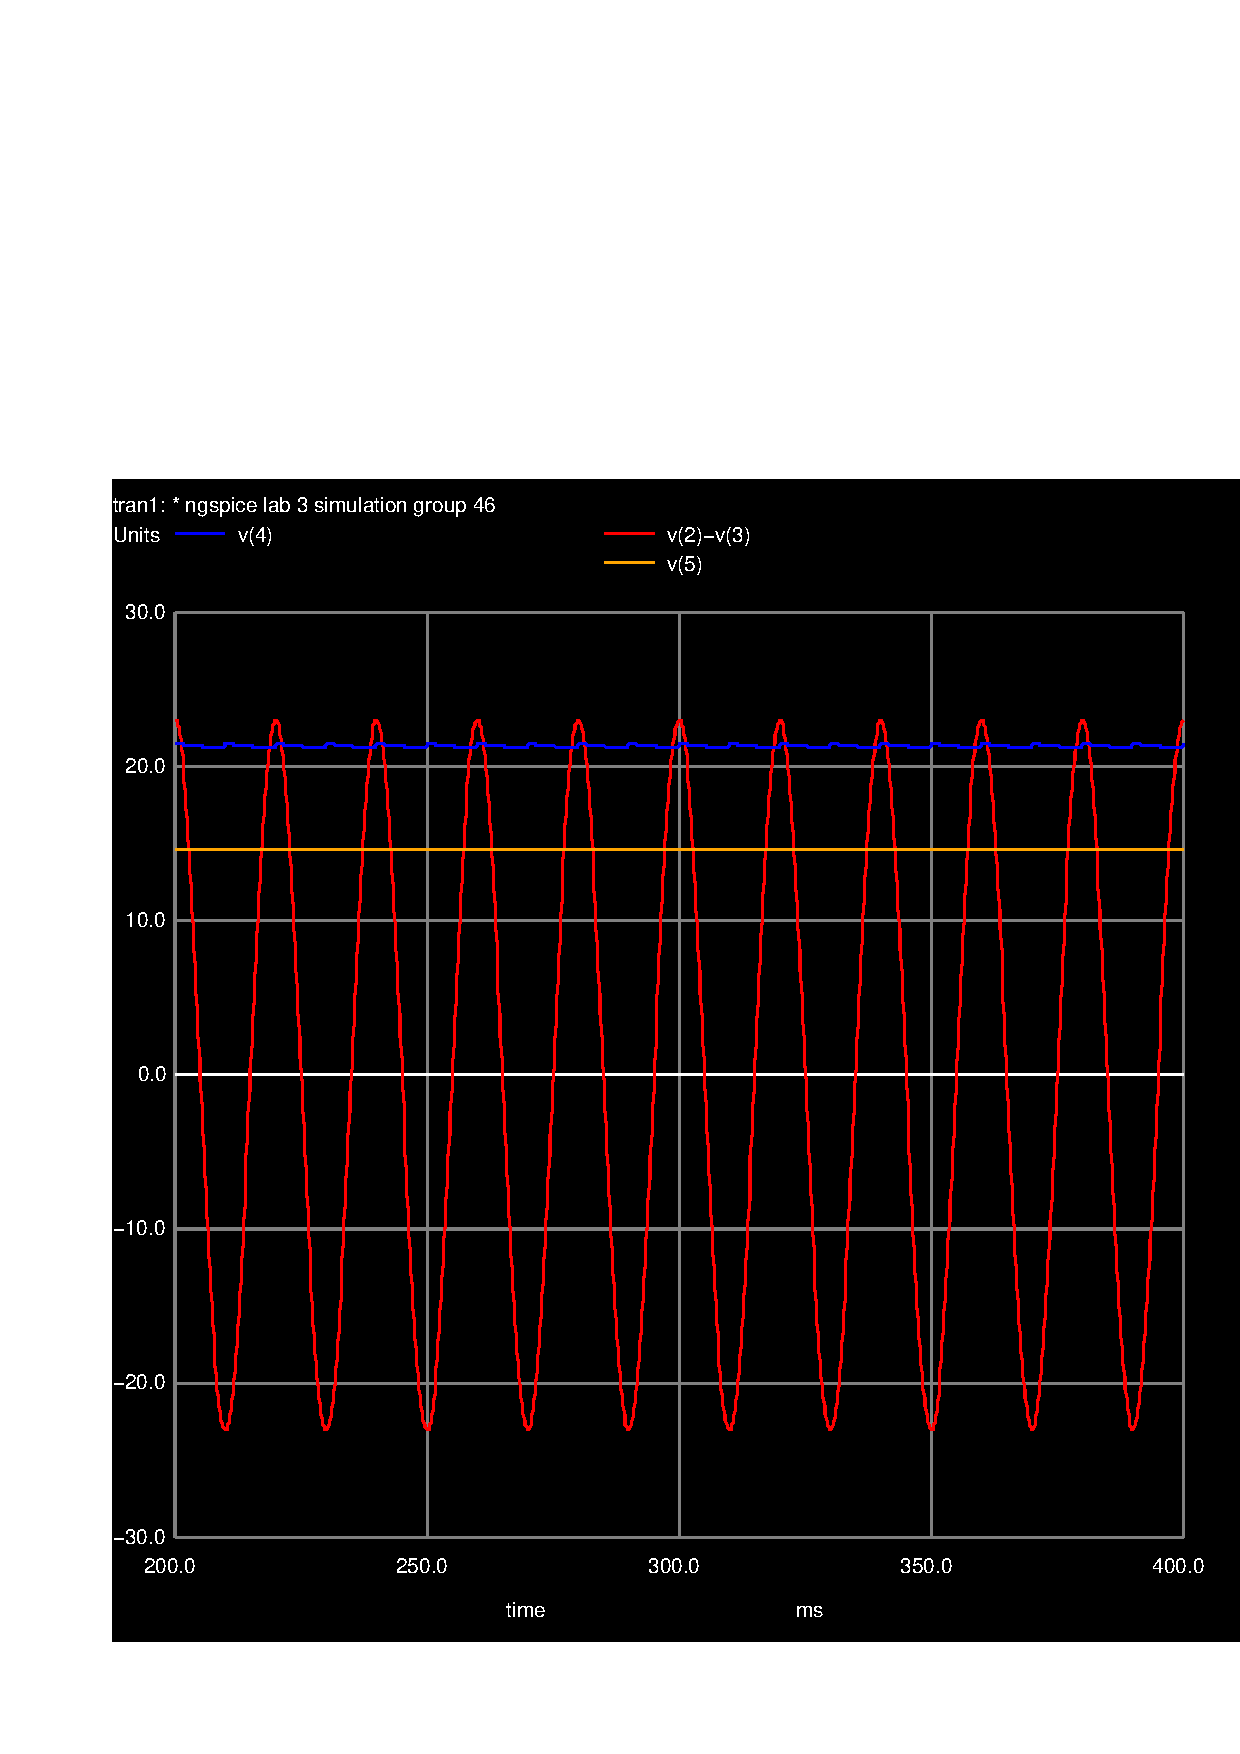
\includegraphics[width=0.6\linewidth]{sim3a.pdf}
	\caption{Input voltage of the dependent voltage source, vr, output voltage of the envelope detector, v(4), and output voltage of the voltage regulator, v(5)}
\label{fig:sim3a}
\end{figure}


This data shows the effect of both the envelope and voltage regulators. The former decreases the ripple voltage and the latter keeps the output voltage constant. While v(5) is not completely a straight line (some oscillations are expected due to the non-linear behavior of the diodes), $v(5) - 12V$ is very close to zero, which was ultimately the main goal of this assignment. 

As one can see in Figure~\ref{fig:sim3b}, the regulated ripple voltage has decreased when compared to the envelope ripple voltage, which indicates that the circuit is operating as expected. 

\begin{figure}[h] \centering
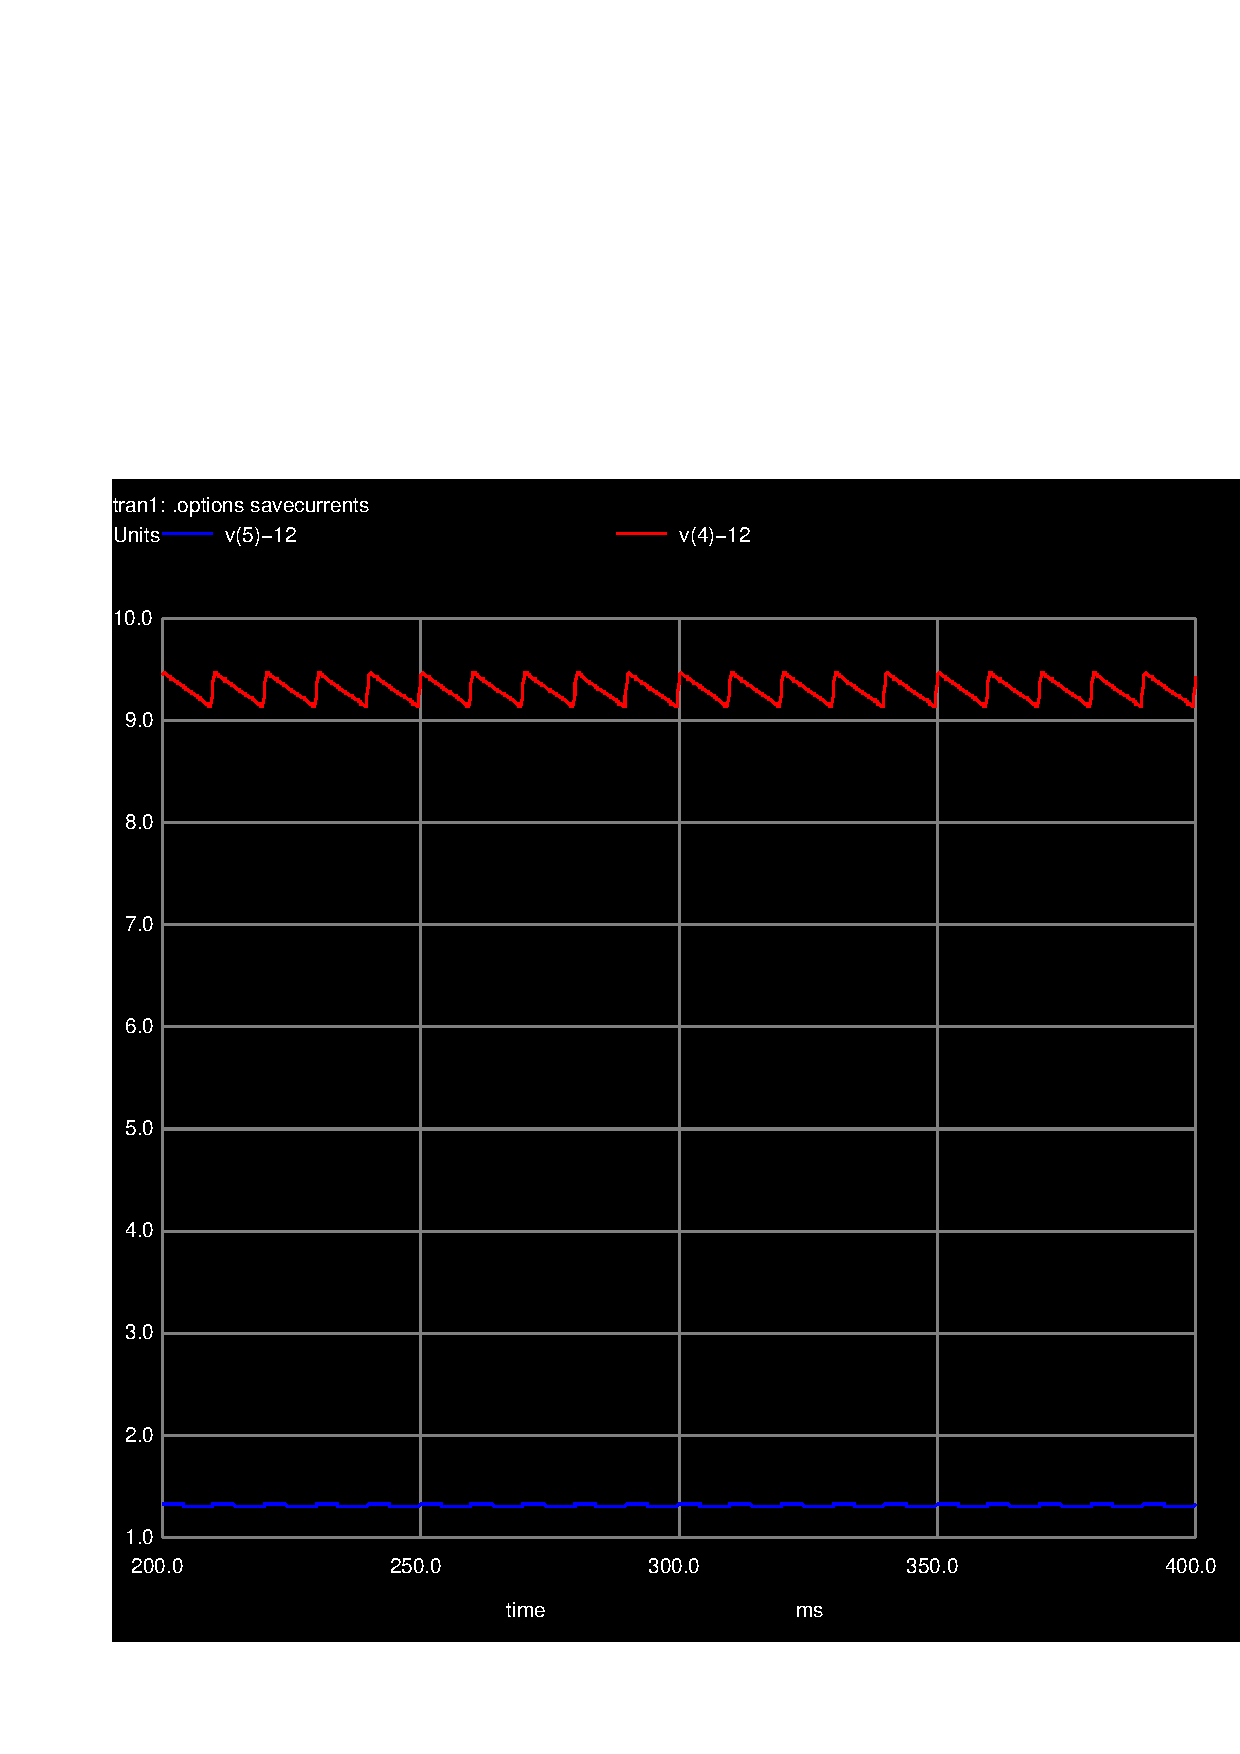
\includegraphics[width=0.6\linewidth]{sim3b.pdf}
	\caption{$v(4)-12V$, $v(5)-12V$}                        
\label{fig:sim3b} 
\end{figure}

The following tables show various values of interest:

\begin{table}[h]
        \parbox{.45\linewidth}{
  \centering
  \begin{tabular}{|l|r|}
    \hline
    {\bf Name} & {\bf Value [V]} \\ \hline
    maximum(v(4))-minimum(v(4)) & 1.741797e-01\\ \hline
mean(v(4)) & 1.276542e+01\\ \hline

  \end{tabular}
  \caption{Envelope ripple and average voltages.}
	\label{tab:env}
}
\hfill
        \parbox{.45\linewidth}{
  \centering
  \begin{tabular}{|l|r|}
    \hline
    {\bf Name} & {\bf Value [V]} \\ \hline
    maximum(v(5))-minimum(v(5)) & 1.933408e-02\\ \hline
mean(v(5)) & 1.331470e+01\\ \hline

  \end{tabular}
  \caption{Regulator ripple and average voltages.}
  \label{tab:reg}
}
\end{table}




